\documentclass{article}
\usepackage[utf8]{inputenc}
\usepackage{graphicx}
\usepackage{amsmath}
\usepackage{listings}
\usepackage{xcolor}
\usepackage{hyperref}
\usepackage{float}
\usepackage[a4paper, top=2cm, bottom=2cm, left=2cm, right=2cm]{geometry}

% Define colors for code syntax highlighting
\lstset{
    language=Java,
    basicstyle=\ttfamily\small,
    keywordstyle=\color{blue},
    stringstyle=\color{red},
    commentstyle=\color{green!50!black},
    numbers=left,
    numberstyle=\tiny,
    stepnumber=1,
    numbersep=10pt,
    showstringspaces=false,
    breaklines=true,
    frame=single,
    captionpos=b
}

\begin{document}

\title{Simulation Model Report: \textbf{FluVirus}}
\author{Author: Rayane GUEROU}
\date{\today}
\maketitle

\begin{abstract}
This report presents the development and analysis of a simulation model named \textbf{FluVirus}, which aims to study how local isolation can reduce the diffusion of an epidemic.
Influenza, commonly known as the "flu," is a contagious respiratory illness caused by influenza viruses. The primary objective of this project is to represent the spread of influenza in an urban environment using GIS data for buildings and roads. \newline

The model simulates daily activities, including commuting between homes and workplaces, and incorporates key factors such as infection probability, recovery rate, and intervention strategies like local isolation and vaccination. Additionally, extensions of the model explore the impacts of family dynamics, virus variants, and vaccination strategies on the spread of the epidemic. The results are presented through plots and detailed discussions.

\end{abstract}

\tableofcontents
\newpage

\section{Introduction}
Influenza, or "flu," is an infectious disease that spreads through respiratory droplets when infected individuals come into contact with healthy people. It can spread rapidly, especially in densely populated urban areas. This project focuses on simulating the dynamics of flu spread in a city, assuming the disease is not fatal, and recovery occurs after a symptomatic period.\newline

Healthy individuals (referred to as Susceptibles) can become infected upon contact with infected individuals. The infection probability in this model is set at 33\%, and recovery can occur either after a fixed period of 10 days or with a 10\% probability per day. Once recovered, individuals do not transmit the disease further.\newline

The main goal of this project is to propose a simulation model that represents flu spread in an urban area using real-world data. The simulation includes daily movement patterns (commuting) and intervention strategies, such as testing and isolating infected individuals. Extensions to the model allow for the inclusion of families, vaccination strategies, and virus variants to further study their impacts.
\newline

\textbf{Key questions addressed include:}
\begin{itemize}
    \item How effective is local isolation in reducing the spread of the epidemic?
    \item What is the impact of varying vaccination rates on epidemic control?
    \item How does the emergence of virus variants affect disease spread and vaccine efficacy?
\end{itemize}


\section{Model Definition}
This chapter provides a detailed explanation of the simulation model implemented using the GAMA modeling language (GAML). The model represents a city environment with buildings and roads, simulates daily commuting patterns, and accounts for key epidemiological factors such as infection and recovery.

\begin{figure}[H]
    \centering
    % Placeholder for the first plot
    
\includegraphics[width=0.8\textwidth]{flu-virus-model.png}
    \caption{[Diagram of the FluVirus Model]}
    \label{fig:plot1}
\end{figure}

This flu virus simulation model represents interactions between key components: \textbf{Buildings}, \textbf{Roads}, \textbf{People}, \textbf{Authorities}, and the \textbf{Virus}. \newline
Inhabitants (\textbf{People}) move through the environment daily using \textbf{Roads} to travel between \textbf{Buildings} where they live, work, or attend school. Authorities are responsible for conducting \textbf{tests} to identify infected individuals and administering \textbf{vaccinations} to reduce the spread of the virus. People can become \textbf{infected} when they come into contact with others who are carrying the virus. Once infected, they may further \textbf{infect neighbors}, contributing to the virus's propagation. \newline
The model simulates daily routines such as going to work, going to school, and returning home, capturing the dynamics of human movement and interaction that drive the epidemic.\newline
\textbf{The diagram highlights these key flows:}
\begin{itemize}
    \item \textbf{Movement} between buildings through roads.
    \item \textbf{Testing and vaccination} efforts by authorities to control the outbreak.
    \item \textbf{Infection transmission} between people and their surroundings.
\end{itemize}

\subsection{global variables \& model initialization}
\begin{lstlisting}[language=Java, caption={Global variables in GAML}]
    shape_file shapefile_buildings <- shape_file("../includes/buildings.shp");
    shape_file shapefile_roads <- shape_file("../includes/roads.shp");

    geometry shape <- envelope(shapefile_roads,shapefile_buildings);
    graph road_network;
    building biggest_building;
    float step <- 5#mn;

    float vaccination_rate <- 0.005;
    int nb_init_people <- 3000;
    int number_infected_init <- 10;
    float infection_probability <- 0.33;
    float mutation_probability <- 0.0005;
    float infection_distance <- 1.0#m;
    float recovery_probability <- 0.1;
    float testing_percentage <- 0.1;
\end{lstlisting}

For the global variables:
\begin{itemize}
    \item \textbf{shape\_file shapefile\_buildings} and \textbf{shape\_file shapefile\_roads} are defined to load the shapefiles for buildings and roads, respectively.
    \item \textbf{geometry shape} is created by enveloping the road and building shapes to represent the overall environment. 
    \item \textbf{graph road\_network} is initialized to represent the network of roads connecting buildings.
    \item \textbf{building biggest\_building} is defined to store the largest building in the environment.
    \item \textbf{float step} is set to 5 minutes to define the step time for the simulation.
    \item \textbf{float vaccination\_rate} is set to 0.005 to define the vaccination rate.
    \item \textbf{int nb\_init\_people} is set to 3000 to define the initial number of people in the simulation.
    \item \textbf{int number\_infected\_init} is set to 10 to define the initial number of infected people in the simulation.
    \item \textbf{float infection\_probability} is set to 0.33 to define the probability of infection.
    \item \textbf{float mutation\_probability} is set to 0.0005 to define the probability of mutation.
    \item \textbf{float infection\_distance} is set to 1.0 meters to define the distance at which infection spreads.
    \item \textbf{float recovery\_probability} is set to 0.1 to define the probability of recovery.
    \item \textbf{float testing\_percentage} is set to 0.1 to define the percentage of people tested for the virus.
\end{itemize}

\begin{lstlisting}[language=Java, caption={Model Initialization in GAML}]
init {
	create virus number: 1 {
		inf_prob <- infection_probability;
	}
	create authorities number: 1;
	create building from: shapefile_buildings;
	biggest_building <- building with_max_of each.shape.area;
	ask biggest_building {
		is_school <- true;
	}
	create road from: shapefile_roads;
	create people number: nb_init_people;
	ask 70 among building {
		is_workplace <- true;
	}
	loop ag over: building where (!each.is_workplace and !each.is_school) {
		int nb_people_family <- rnd(3,6);
		int nb_kids_family <- rnd(0,2);
		ask (nb_people_family - nb_kids_family) among (people where (each.house = nil)) {
			house  <- ag;
			workplace <- one_of(building where (each.is_workplace));
			location <- any_location_in(house);
		}
		ask nb_kids_family among (people where (each.house = nil)) {
			is_child <- true;
			house  <- ag;
			school <- one_of(biggest_building);
			location <- any_location_in(house);
		}
	}	
	ask number_infected_init among people {
		is_infected <- true;
		VIRUS <- one_of(virus);
		all_virus_contracted << VIRUS;
	}	
	road_network <- as_edge_graph(road);	
}   
\end{lstlisting}

The model initialization process includes the following steps:
\begin{itemize}
    \item \textbf{create virus number: 1} creates a single instance of the virus.
    \item \textbf{create authorities number: 1} creates a single instance of the authorities.
    \item \textbf{create building from: shapefile\_buildings} creates building instances from the provided shapefile.
    \item \textbf{biggest\_building $\leftarrow$ building with\_max\_of (each.shape.area)} identifies the largest building in the environment.
    \item \textbf{ask biggest\_building} sets the largest building as a school.
    \item \textbf{create road from: shapefile\_roads} creates road instances from the provided shapefile.
    \item \textbf{create people number: nb\_init\_people} creates people instances.
    \item \textbf{ask 70 among building {is\_workplace $\leftarrow$ true}} sets 70 of the buildings as workplaces, so people don't go to work in others family house, we create 70 uniques workplaces were all the people will go to work.
    \item \textbf{loop ag over: building where (!each.is\_workplace and !each.is\_school)} iterates over all buildings that are neither workplaces nor schools.
    \item \textbf{int nb\_people\_family $\leftarrow$ rnd(3,6)} generates a random number of people in the family.
    \item \textbf{int nb\_kids\_family $\leftarrow$ rnd(0,2)} generates a random number of kids in the family.
    \item \textbf{ask (nb\_people\_family - nb\_kids\_family) among (people where (each.house = nil))} assigns people to households, we don't forget to exclude the kids from this loop by subtracting nb\_kids\_family.
    \item \textbf{ask nb\_kids\_family among (people where (each.house = nil))} assigns kids to schools.
\end{itemize}
I have created a reflex to stop the simulation when there are no more infected people in the simulation, to avoid running the simulation indefinitely.

\subsection{Species Virus}
\begin{lstlisting}[language=Java, caption={Species Virus in GAML}]
species virus {
    float inf_prob;
}
\end{lstlisting}
This species represents the virus in the simulation, with the \textbf{inf\_prob} attribute defining the infection probability. It was created to store the virus properties, which change with every virus mutation, and to keep track of which people have been infected by which virus, and to permit the authorities to see which virus is the more spread to give people the right vaccine.

\subsection{Species Building}
\begin{lstlisting}[language=Java, caption={Species Building in GAML}]
species building {
    bool is_school <- false;
    bool is_workplace <- false;
    
    aspect default {
        draw shape color: #darkgray;
    }
}
\end{lstlisting}
This species represents buildings in the simulation, with attributes \textbf{is\_school} and \textbf{is\_workplace} to differentiate between schools and workplaces. The aspect default defines the appearance of buildings in the simulation.

\subsection{Species Road}
\begin{lstlisting}[language=Java, caption={Species Road in GAML}]
species road {
    aspect default {
        draw shape color: #lightgray;
    }
}
\end{lstlisting}
This species represents roads in the simulation, with the aspect default defining the appearance of roads in the simulation.

\subsection{Species Authorities}
\begin{lstlisting}[language=Java, caption={Species Authorities Parameters in GAML}]
map<virus,int> list_virus;
int max_value <- 0;
virus VACCIN_URGENCE;
\end{lstlisting}
This species represents the authorities in the simulation, responsible for conducting tests and administering vaccines to control the epidemic.
The attributes \textbf{list\_virus} and \textbf{max\_value} are used to track the number of people infected by each virus and identify the most prevalent virus.
The attribute \textbf{VACCIN\_URGENCE} stores the virus for which a vaccine is urgently needed.

\begin{lstlisting}[language=Java, caption={Authorities Reflexes in GAML}]
    reflex vaccination when: world.time mod 86400 = 25200 {
		ask int(vaccination_rate * nb_init_people) among (people where(not(each.all_vaccine contains VACCIN_URGENCE))) {
			is_vaccinated <- true;
			VACIN <- myself.VACCIN_URGENCE;
			all_vaccine << myself.VACCIN_URGENCE;
		}
	}
\end{lstlisting}
This reflex is made to handle the vaccination process. It is triggered at 7:00 AM, and it vaccinates a percentage of the population with the vaccine for the most prevalent virus. People can only be vaccinated once, and they receive the vaccine for the most prevalent virus.

\begin{lstlisting}[language=Java, caption={Authorities Reflexes in GAML}]
reflex testing when: world.time mod 86400 = 25200 {
    ask int(testing_percentage * nb_init_people) among (people where(!each.is_isolated)) {
        if (is_infected) {
            is_isolated <- true;
        }
    }
}
\end{lstlisting}
This reflex is made to handle the testing process. It is triggered at 7:00 AM, and it tests a percentage of the population for the virus. If the person is infected, they are isolated to prevent further spread of the virus.

\begin{lstlisting}[language=Java, caption={Authorities new Vaccine in GAML}]
reflex counting when: world.time mod 86400 = 25200 {
    loop ag over: virus {
        list_virus[ag] <- people count (each.VIRUS = ag);
        if (list_virus[ag] > max_value) {
            max_value <- list_virus[ag];
            VACCIN_URGENCE <- ag;
        }
    }
    write(list_virus);
    max_value <- 0;
}
\end{lstlisting}
This reflex is made to handle the counting of infected people by virus. It is triggered at 7:00 AM, and it counts the number of people infected by each virus. The virus with the highest number of infections is identified as the most prevalent virus, and the authorities prepare a vaccine for it.


\subsection{Species People}
\begin{lstlisting}[language=Java, caption={Parameters of People in GAML}]
point target;
building house;
building workplace;
building school;
bool is_child;
virus VIRUS;
list<virus> all_virus_contracted;
virus VACIN;
list<virus> all_vaccine;

int recovery_time <- 0;
int isolated_time <- 0;
bool is_infected <- false;
bool is_vaccinated <- false;
bool is_isolated <- false;
float infect_prob <- infection_probability;

rgb color -> is_infected ? #red : #green;
list<people> neighbours -> people at_distance infection_distance;
\end{lstlisting}
The species People represents individuals in the simulation, with attributes such as \textbf{house}, \textbf{workplace}, \textbf{school}, \textbf{is\_child}, \textbf{VIRUS}, \textbf{all\_virus\_contracted}, \textbf{VACIN}, and \textbf{all\_vaccine} to track their status, location, and interactions. The attributes \textbf{recovery\_time}, \textbf{isolated\_time}, \textbf{is\_infected}, \textbf{is\_vaccinated}, \textbf{is\_isolated}, and \textbf{infect\_prob} are used to model infection, recovery, vaccination, and isolation processes. The \textbf{color} attribute is used to visualize the infection status of individuals, with red representing infected and green representing healthy individuals. The \textbf{neighbours} attribute stores the list of people within the infection distance of each individual.

\begin{lstlisting}[language=Java, caption={Update Infection Probability in GAML}]
reflex infection_prob when: (VIRUS != nil) {
    infect_prob <- VIRUS.inf_prob;
    if (is_vaccinated) {
        infect_prob <- infect_prob/3;
        if (all_vaccine contains VIRUS) {
            
        } else {
            infect_prob <- infect_prob * 2;
        }
    }
}
\end{lstlisting}
This reflex is made to handle the evolution of the infection probability of a person, depending on the virus they have contracted and the vaccine they have received. If the person is vaccinated, the infection probability is reduced by a factor of 3, and if the person has not received the good vaccine, the infection probability is increased by a factor of 2. If he is not vaccinated, the infection probability is the same as the virus infection probability.

\begin{lstlisting}[language=Java, caption={People Isolation and Recovering in GAML}]
reflex isolation when: (world.time mod 86400 = 25200 and is_isolated) {
    if (isolated_time = 12) {
        is_isolated <- false;
        isolated_time <- 0;
    }
    isolated_time <- isolated_time + 1;
}

reflex recover when: (world.time mod 86400 = 25200 and is_infected) {
    if (recovery_time = 10 or flip(recovery_probability)) {
        is_infected <- false;
        recovery_time <- 0;
        VIRUS <- nil;
    } else {
	recovery_time <- recovery_time + 1;
    }
}	
\end{lstlisting}
These reflexes are made to handle the isolation and recovery of people. The isolation reflex checks if the person has been isolated for 12 days, and if so, it stops the isolation. The recovery reflex checks if the person has been infected for 10 days or if the recovery probability is met, and if so, it stops the infection.

\begin{lstlisting}[language=Java, caption={People Movement in GAML}]
reflex gowork when: (world.time mod 86400 = 32400 and !is_isolated) {
	if (is_child) {
		target <- any_location_in(school);
	} else {
		target <- any_location_in(workplace);
	}
}
	
reflex gohome when: (world.time mod 86400 = 61200 and !is_isolated) {
    target <- any_location_in(house);
}
reflex move when: target != nil {
	do goto target: target on: road_network;
	if(location = target) {
		target <- nil;
	}
}
\end{lstlisting}
These reflexes are made to handle the daily movement of people. The gowork reflex is triggered at 9:00 AM, and it sets the target location to the school for children and the workplace for adults. The gohome reflex is triggered at 6:00 PM, and it sets the target location to the person's house. The move reflex moves the person towards the target location using the road network.

\begin{lstlisting}[language=Java, caption={Virus Mutation in GAML}]
reflex mutation when: (world.time mod 86400 = 25200 and flip(mutation_probability) and is_infected){
	create virus number: 1{
		inf_prob <- infection_probability * rnd(0.5,1.5);
	}
	VIRUS <- last(virus);
	all_virus_contracted << VIRUS;
}
\end{lstlisting}
This reflex is made to handle the mutation of the virus. It is triggered at 7:00 AM, and if the mutation probability is met, a new virus is created with a random infection probability between 0.5 and 1.5 times the original infection probability. The person is then infected with the new virus.

\begin{lstlisting}[language=Java, caption={People Infection in GAML}]
reflex become_infected when: (is_infected and flip(infect_prob)){
    ask neighbours {
        if (all_virus_contracted contains myself.VIRUS) {
            
        } else {
            all_virus_contracted << myself.VIRUS;
            is_infected <- true;
            VIRUS <- myself.VIRUS;
        }
    }
}
\end{lstlisting}
This reflex is made to handle the infection of people. If the person is infected and the infection probability is met, the person can infect their neighbors if they have not already been infected by the same virus.

\section{Simulation Parameters}
\begin{lstlisting}[language=Java, caption={Simulation Parameters in GAML}]
parameter "Nb people" var: nb_init_people step:100 max: 3100;
parameter "Vaccination rate" var: vaccination_rate min:0 max: 1.0;
parameter "Infection distance" var: infection_distance;	
parameter "Probaibilty of infection" var: infection_probability min:0 max: 1.0;
parameter "Probaibilty of virus mutation" var: mutation_probability min:0 max: 1.0;
parameter "Distance of infection" var: infection_distance ;
parameter "Probaibilty of recovery" var: recovery_probability min:0 max: 1.0;
parameter "Testing rate" var: testing_percentage min:0 max: 1.0;
\end{lstlisting}
These parameters are defined to allow users to interact with the simulation and explore the effects of varying vaccination rates, infection probabilities, mutation probabilities, recovery probabilities, and testing rates on the spread of the virus.
In the next sections we will see how these parameters are used in the simulation, to see how they affect the spread of the virus.



\section{Results}
This section presents the results of the simulation model, focusing on the spread of the virus in an urban environment and the effectiveness of intervention strategies such as local isolation and vaccination.

\subsection{Analysis of Simulation Results Without Intervention}
The simulation results presented in Figure 2 illustrate the dynamics of flu virus propagation in an urban environment without any intervention measures—no testing, no isolation, and no vaccination.

\paragraph{No-intervention scenario}
In the absence of any control measures, the virus spreads rapidly, leading to a high number of infections in a short period. The infection curve exhibits multiple large peaks over time, indicating repeated waves of outbreaks. With no vaccination to reduce susceptibility or testing to identify and isolate infected individuals, the entire population remains vulnerable, and the virus propagates unchecked.

\begin{figure}[H]
    \centering
    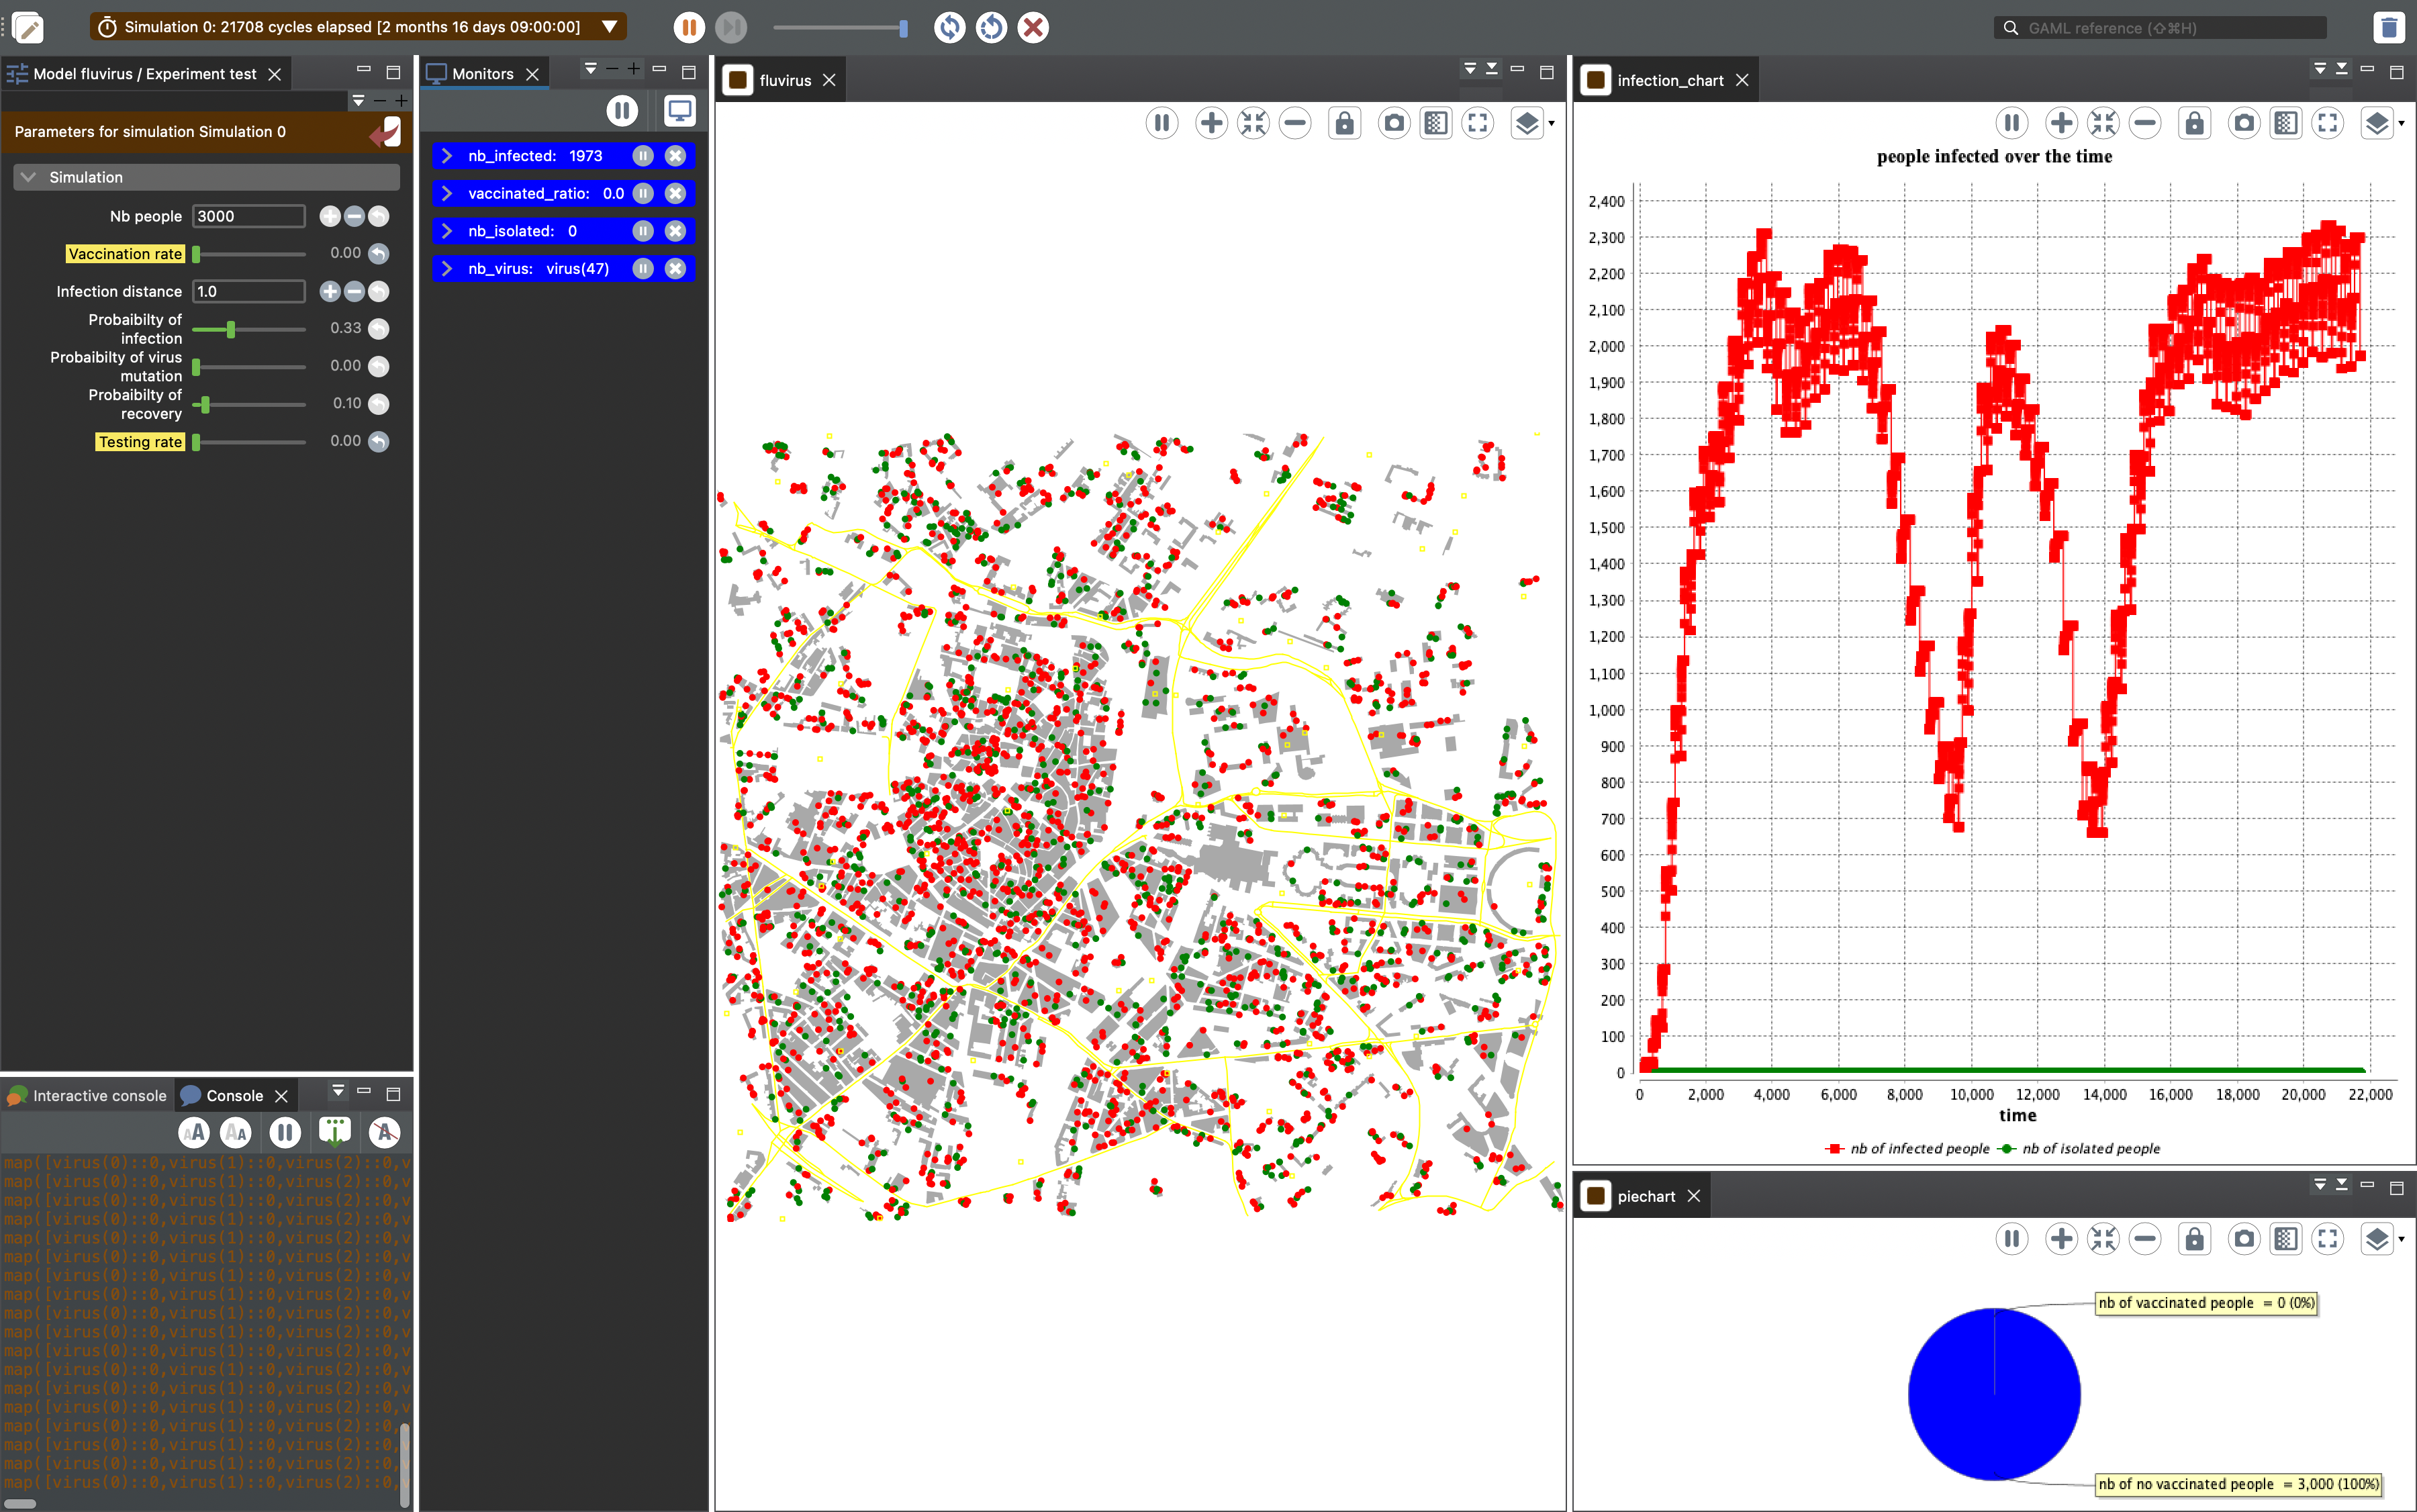
\includegraphics[width=0.8\textwidth]{images/simulation_test.png}
    \caption{Simulation results without intervention: no vaccination, testing, or isolation.}
    \label{fig:no_intervention}
\end{figure}

\paragraph{Key observations}
\begin{itemize}
    \item \textbf{Rapid spread}: Without intervention, the virus quickly infects a large proportion of the population, resulting in several pronounced peaks in the infection curve.
    \item \textbf{High infection rate}: The absence of vaccination and isolation leads to a high infection rate, with nearly the entire population getting infected at some point during the simulation.
    \item \textbf{Recurring outbreaks}: The multiple peaks observed suggest that, in the absence of control measures, the epidemic experiences recurring waves, as recovered individuals eventually become susceptible again due to model dynamics.
\end{itemize}
This scenario highlights the critical importance of intervention strategies such as vaccination, testing, and isolation in controlling an epidemic. Without these measures, the virus spreads rapidly, leading to large-scale outbreaks and significant public health impacts. This underscores the need for timely and effective interventions to mitigate the spread of infectious diseases.

\subsection{Normal Simulation}
\begin{figure}[H]
    \centering
    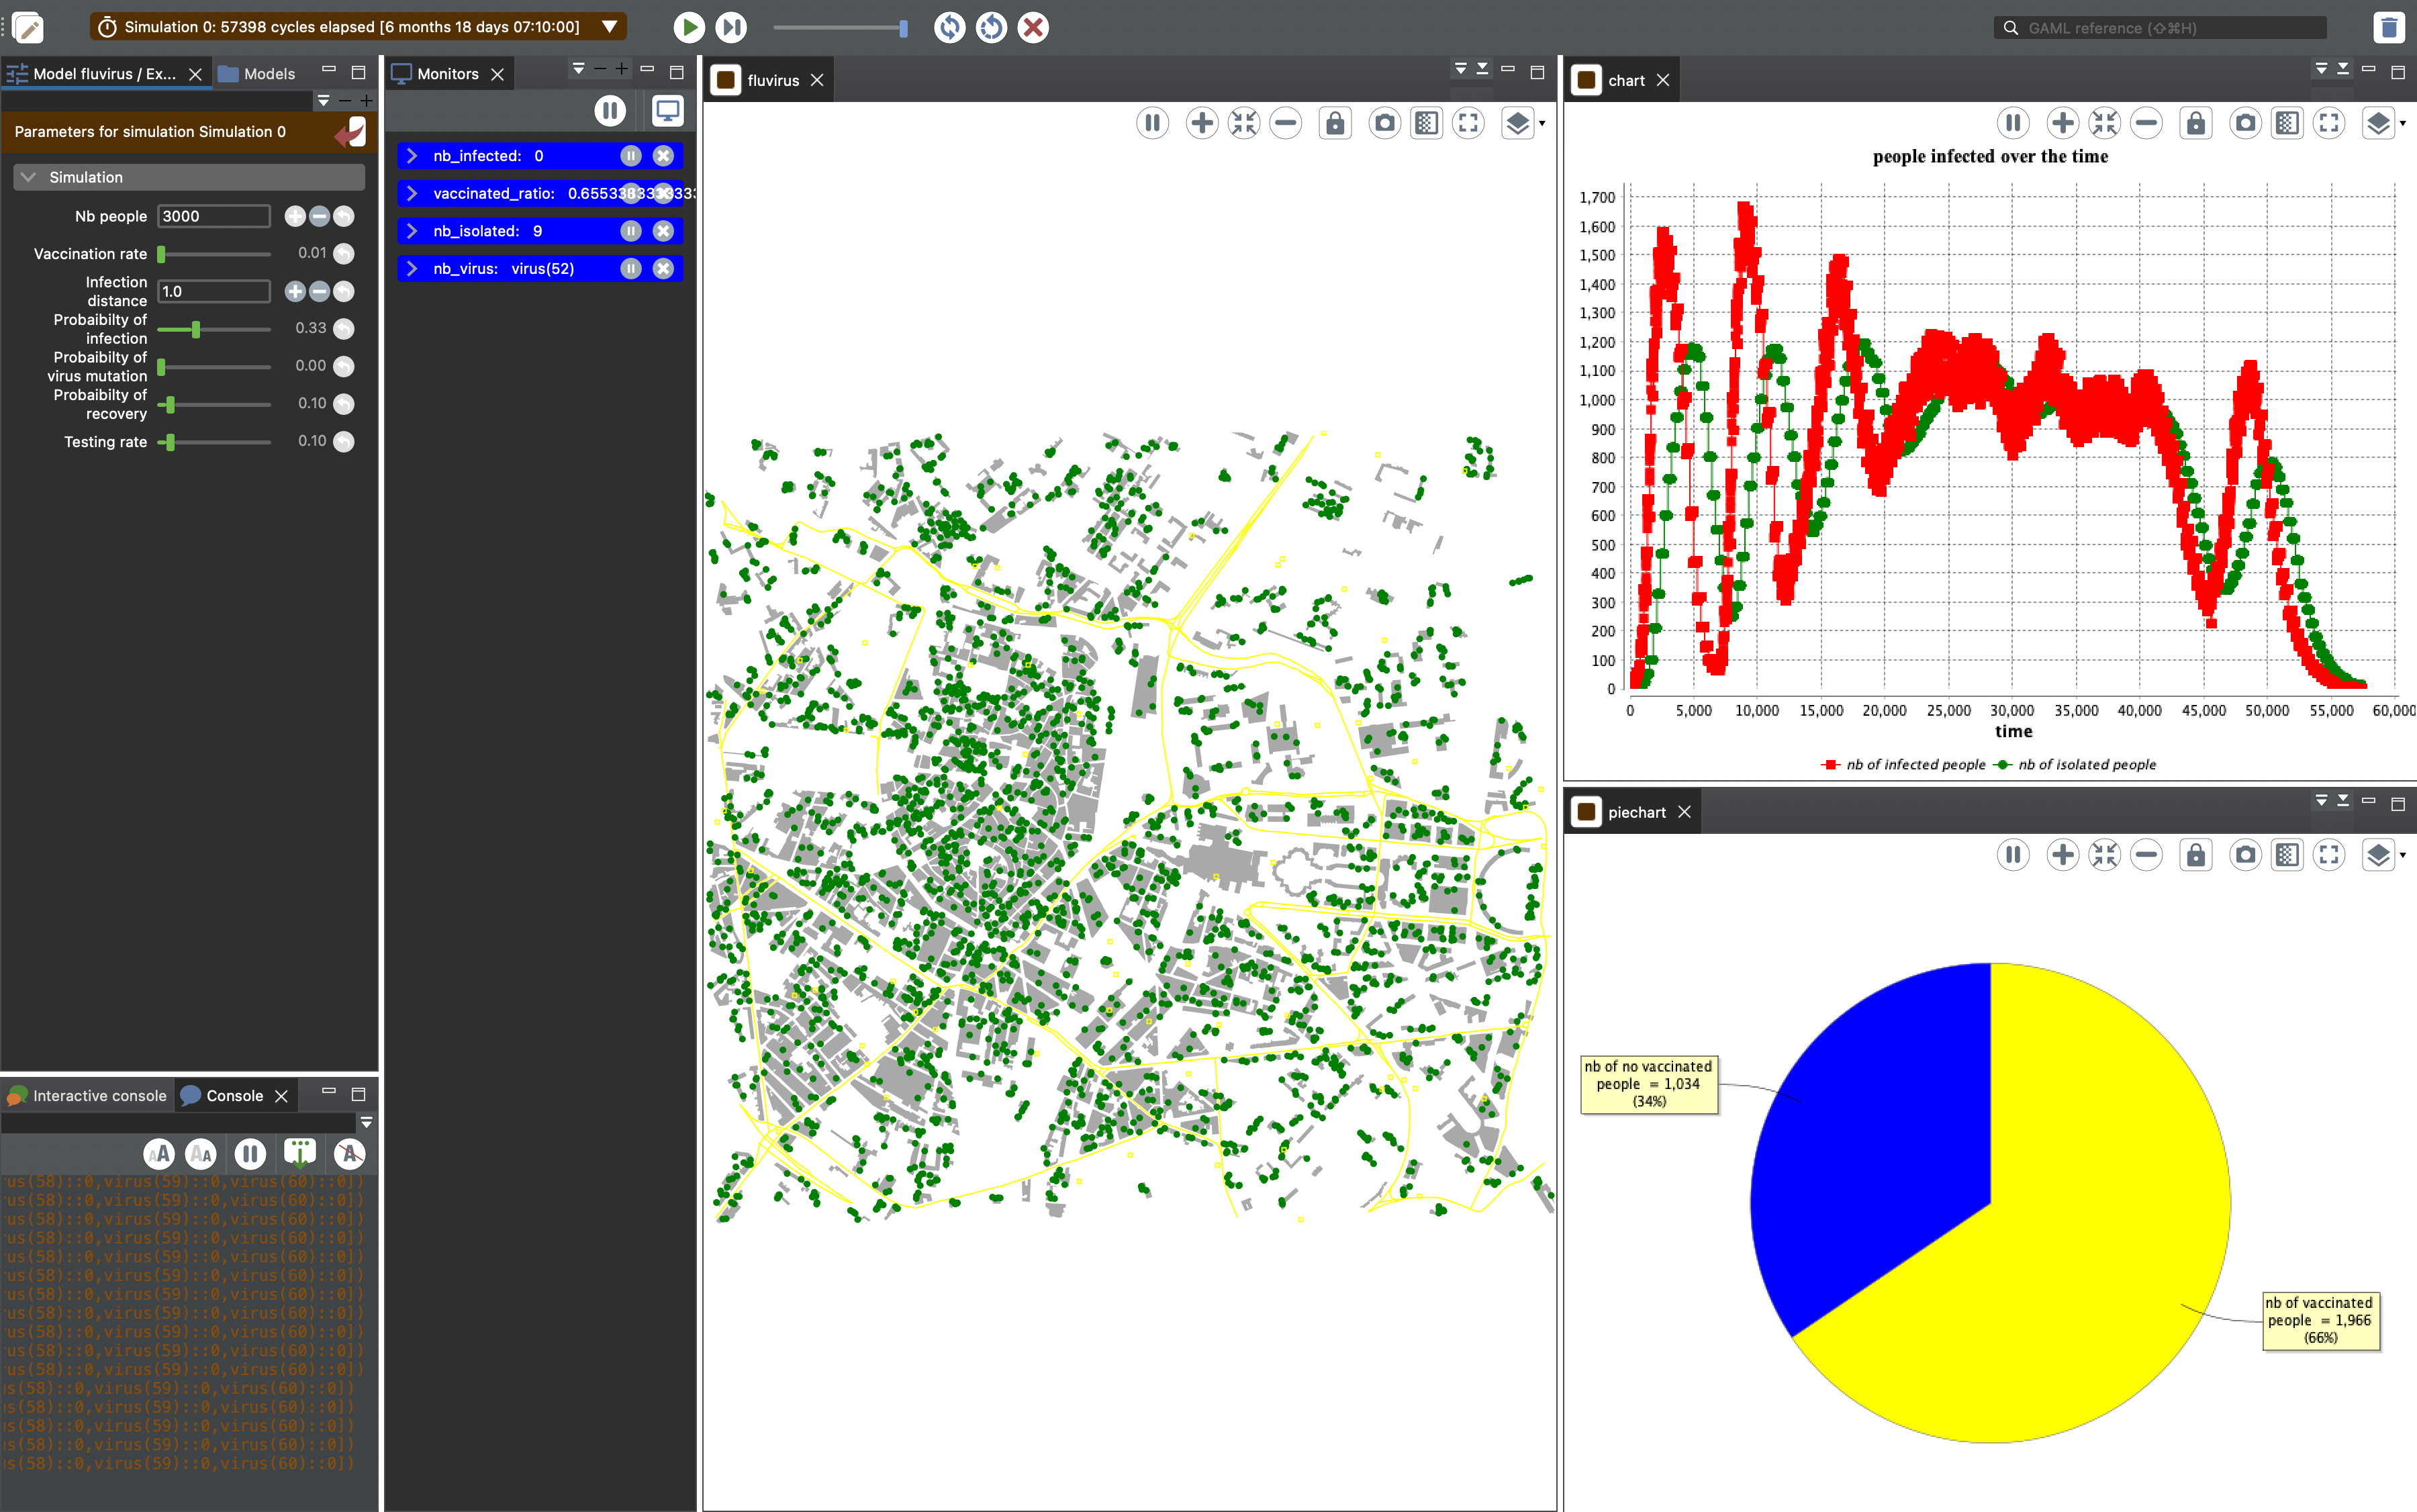
\includegraphics[width=0.8\textwidth]{images/simulation_normal.png}
    \caption{[Description of Plot]}
    \label{fig:plot2}
\end{figure}
The graph on the top right shows the number of infected people and isolated individuals over time. Initially, the number of infected individuals rises sharply as the virus spreads quickly among the susceptible population. Peaks in the infection curve correspond to moments when transmission is at its highest. Over time, as isolation measures and vaccinations take effect, the number of infections begins to stabilize and eventually decreases. This suggests that isolation policies and vaccination campaigns play a crucial role in controlling the outbreak.

The pie chart on the bottom right shows the proportion of vaccinated versus non-vaccinated individuals. With approximately 66\% of the population vaccinated, the simulation demonstrates a significant reduction in infection spread compared to an entirely susceptible population. However, the remaining 34\% of unvaccinated individuals still represent a risk for continued transmission and potential future outbreaks.

\paragraph{Key observations:}
\begin{itemize}
    \item \textbf{Initial spread}: The rapid rise in infections at the start highlights the importance of early intervention measures.
    \item \textbf{Vaccination effect}: A vaccination coverage of 66\% reduces the infection rate but does not entirely eliminate the spread, indicating the need for higher coverage or complementary strategies.
    \item \textbf{Isolation}: The isolated population closely follows the trend of infected individuals, showing the effectiveness of identifying and isolating infected people to limit transmission.
\end{itemize}

Overall, the simulation highlights that while vaccination and isolation reduce the spread of the flu virus, achieving a high vaccination seems to be crucial for long-term epidemic control.

\subsection{Analysis of Simulation Results with No Vaccination}
The two simulations presented in Figures 4 and 5 illustrate the spread of the flu virus in an urban environment under different daily testing rates (20\% and 30\%) without any vaccination.

\paragraph{Simulation with 20\% testing rate}
In Figure 4, the infection curve shows a sharp increase in the number of infected individuals at the start, followed by a gradual decline after reaching a peak. The testing rate of 20\% allows authorities to isolate a significant number of infected individuals, which slows down the spread of the virus. However, the absence of vaccination means that a large proportion of the population still becomes infected over time.

\begin{figure}[H]
    \centering
    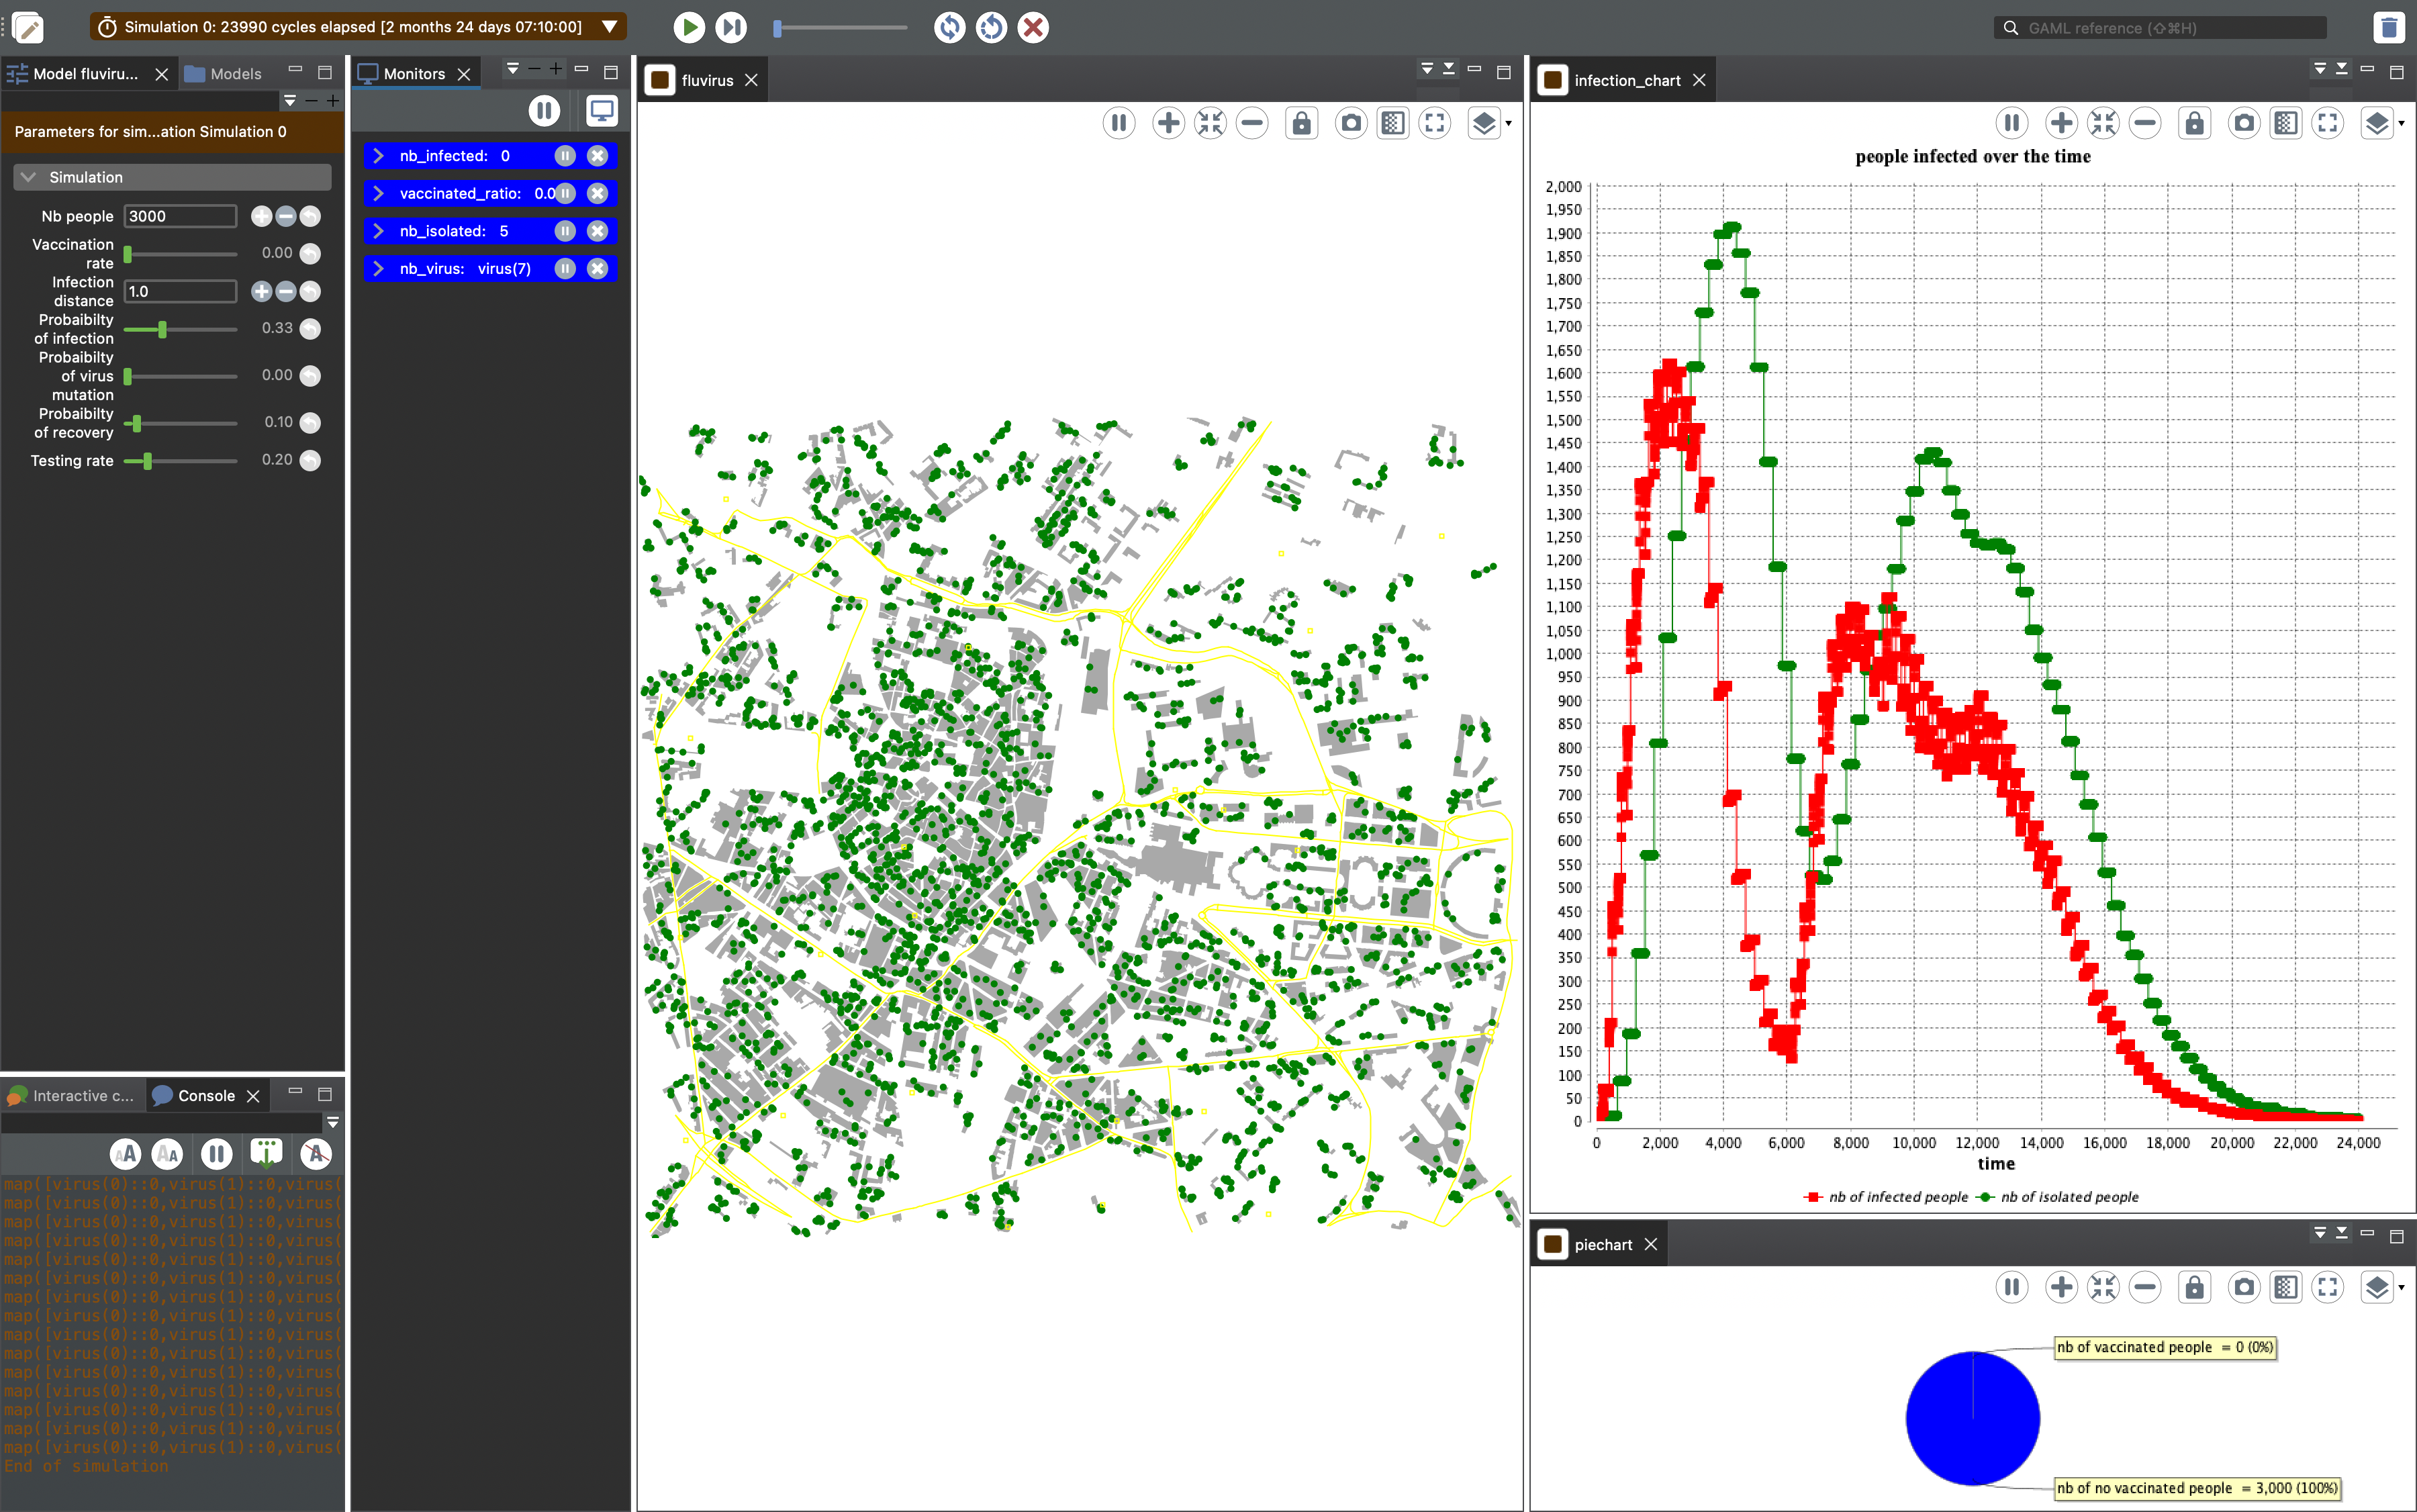
\includegraphics[width=0.8\textwidth]{images/simulation_no_vaccination.png}
    \caption{Simulation results with no vaccination and a daily testing rate of 20\%.}
    \label{fig:simulation_no_vaccination_20}
\end{figure}

\paragraph{Simulation with 30\% testing rate}
In Figure 5, increasing the daily testing rate to 30\% results in a faster decline in the number of infected individuals after the peak. This higher testing rate allows authorities to identify and isolate more infected people earlier, effectively reducing transmission. The epidemic curve is narrower, indicating a shorter epidemic duration compared to the 20\% testing scenario.

\begin{figure}[H]
    \centering
    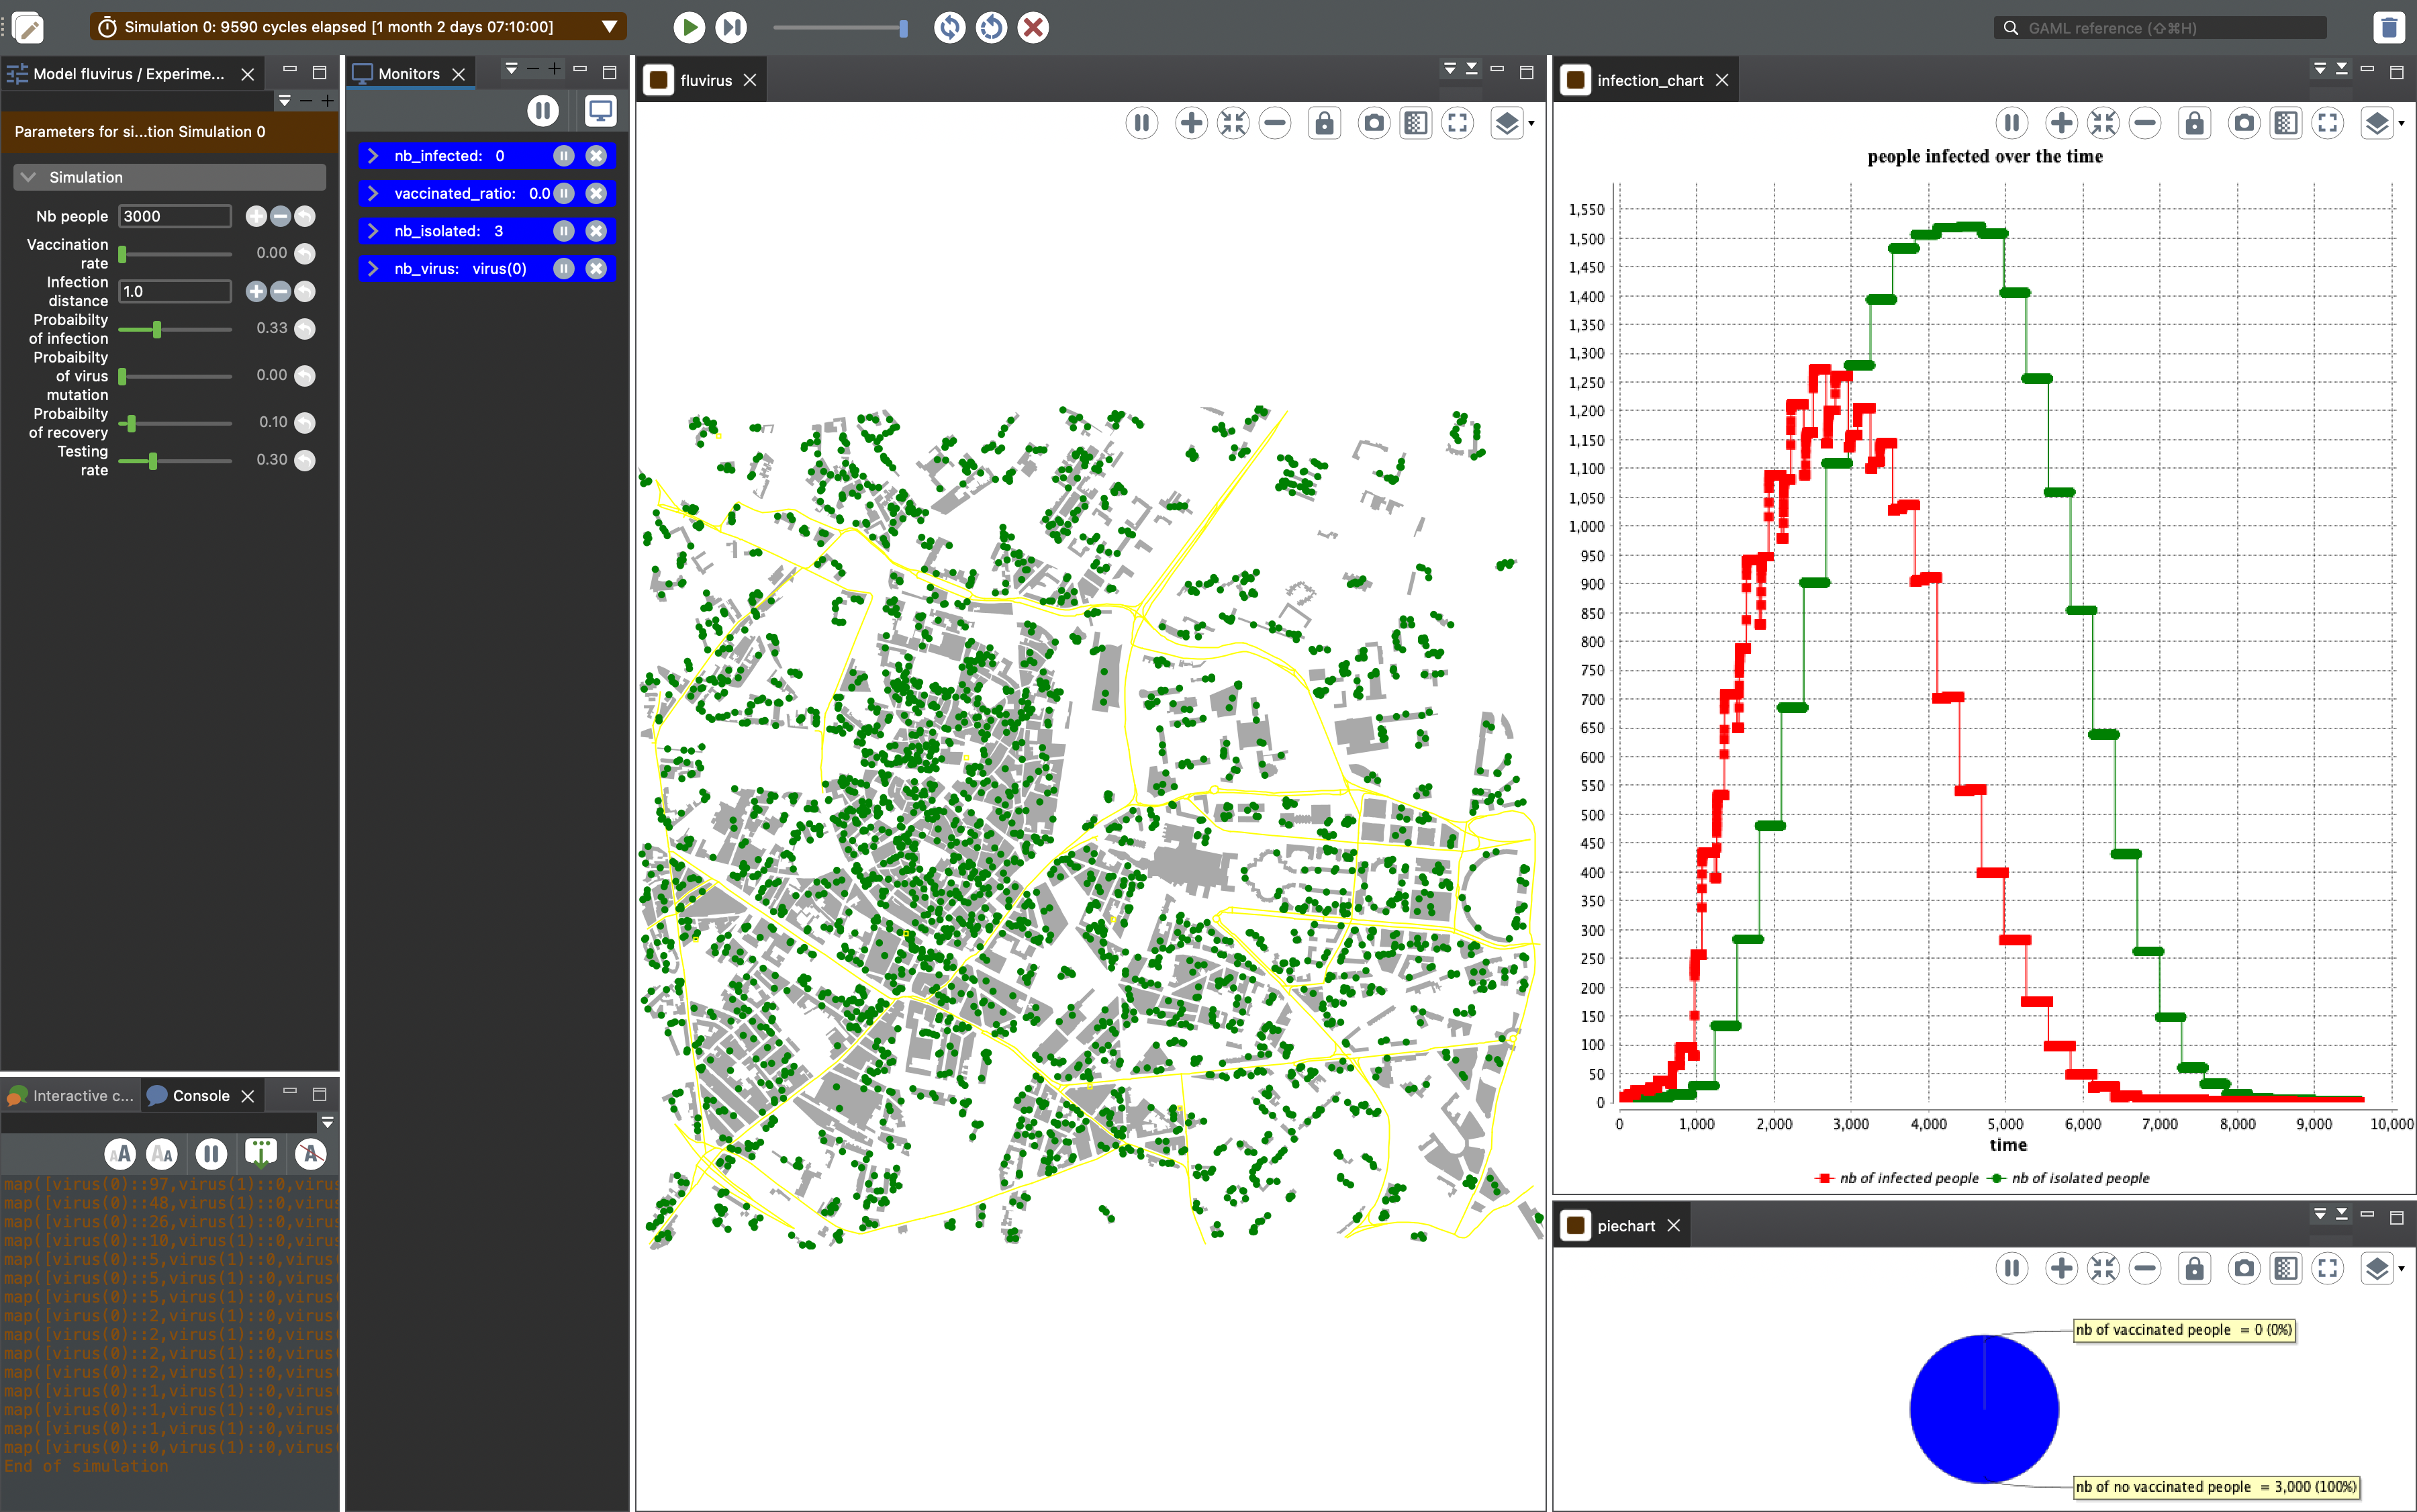
\includegraphics[width=0.8\textwidth]{images/simulation_no_vaccinationv2.png}
    \caption{Simulation results with no vaccination and a daily testing rate of 30\%.}
    \label{fig:simulation_no_vaccination_30}
\end{figure}

\paragraph{Key observations}
\begin{itemize}
    \item \textbf{Impact of testing rate}: A higher testing rate leads to faster isolation of infected individuals, which significantly reduces the spread and shortens the epidemic duration.
    \item \textbf{Effectiveness without vaccination}: Even without vaccination, increasing the testing rate is an effective strategy to control the epidemic, although it cannot prevent large-scale infections.
    \item \textbf{Need for complementary strategies}: The results suggest that while testing and isolation help control the spread, vaccination would be necessary to further reduce the total number of infections and prevent future outbreaks.
\end{itemize}

Overall, these simulations show the importance of early detection and isolation in controlling an epidemic, especially when vaccination is not available.

\subsection{Analysis of Simulation Results with Vaccination and No Isolation}
The simulations presented in Figures 6 and 7 demonstrate the impact of different vaccination rates (5\% and 10\%) on the spread of the flu virus in an urban environment without isolation measures.

\paragraph{Simulation with 5\% vaccination rate}
In Figure 6, with a vaccination rate of 5\%, the infection curve fluctuates significantly over time, showing several peaks. The absence of isolation measures allows the virus to spread rapidly among susceptible individuals. Despite a small reduction in the number of infections compared to a scenario with no vaccination, the low vaccination rate is insufficient to prevent large-scale outbreaks.

\begin{figure}[H]
    \centering
    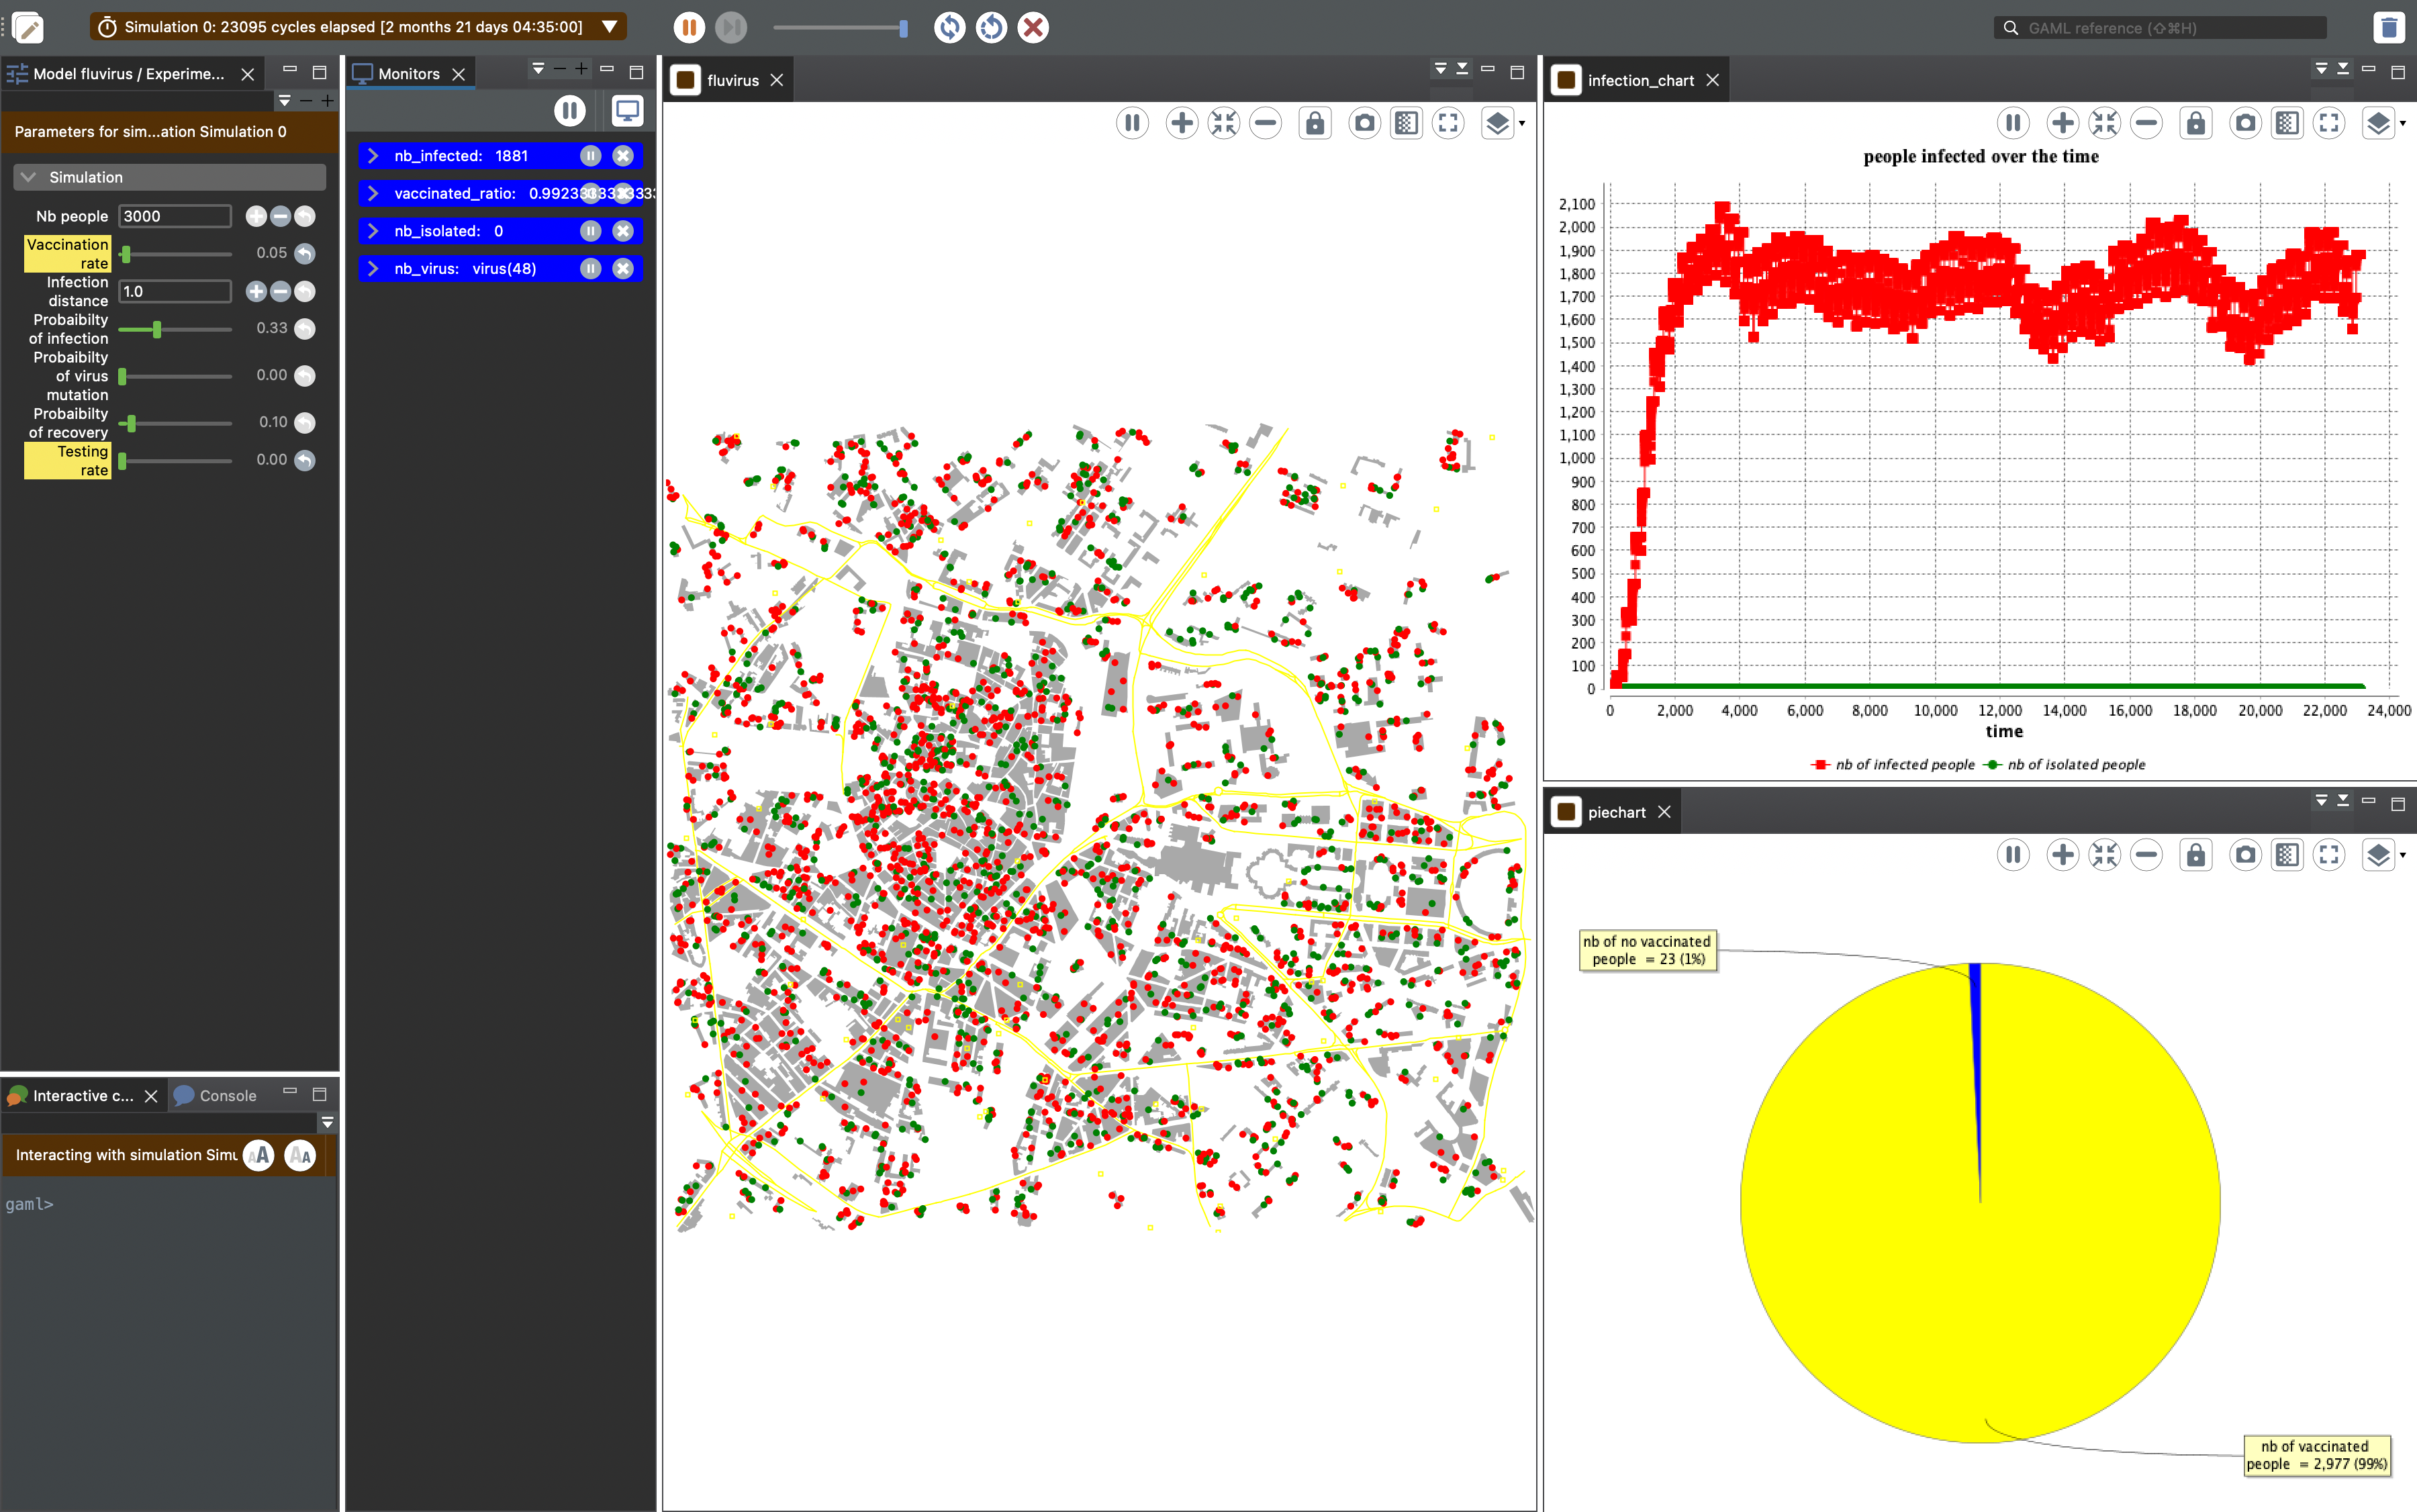
\includegraphics[width=0.8\textwidth]{images/image.png}
    \caption{Simulation results with a 5\% vaccination rate and no isolation.}
    \label{fig:simulation_vaccination_5}
\end{figure}

\paragraph{Simulation with 10\% vaccination rate}
In Figure 7, increasing the vaccination rate to 10\% results in a slight improvement. The infection curve shows fewer and less pronounced peaks, indicating that a higher proportion of vaccinated individuals helps reduce transmission. However, without isolation, the virus continues to spread, leading to repeated outbreaks over time.

\begin{figure}[H]
    \centering
    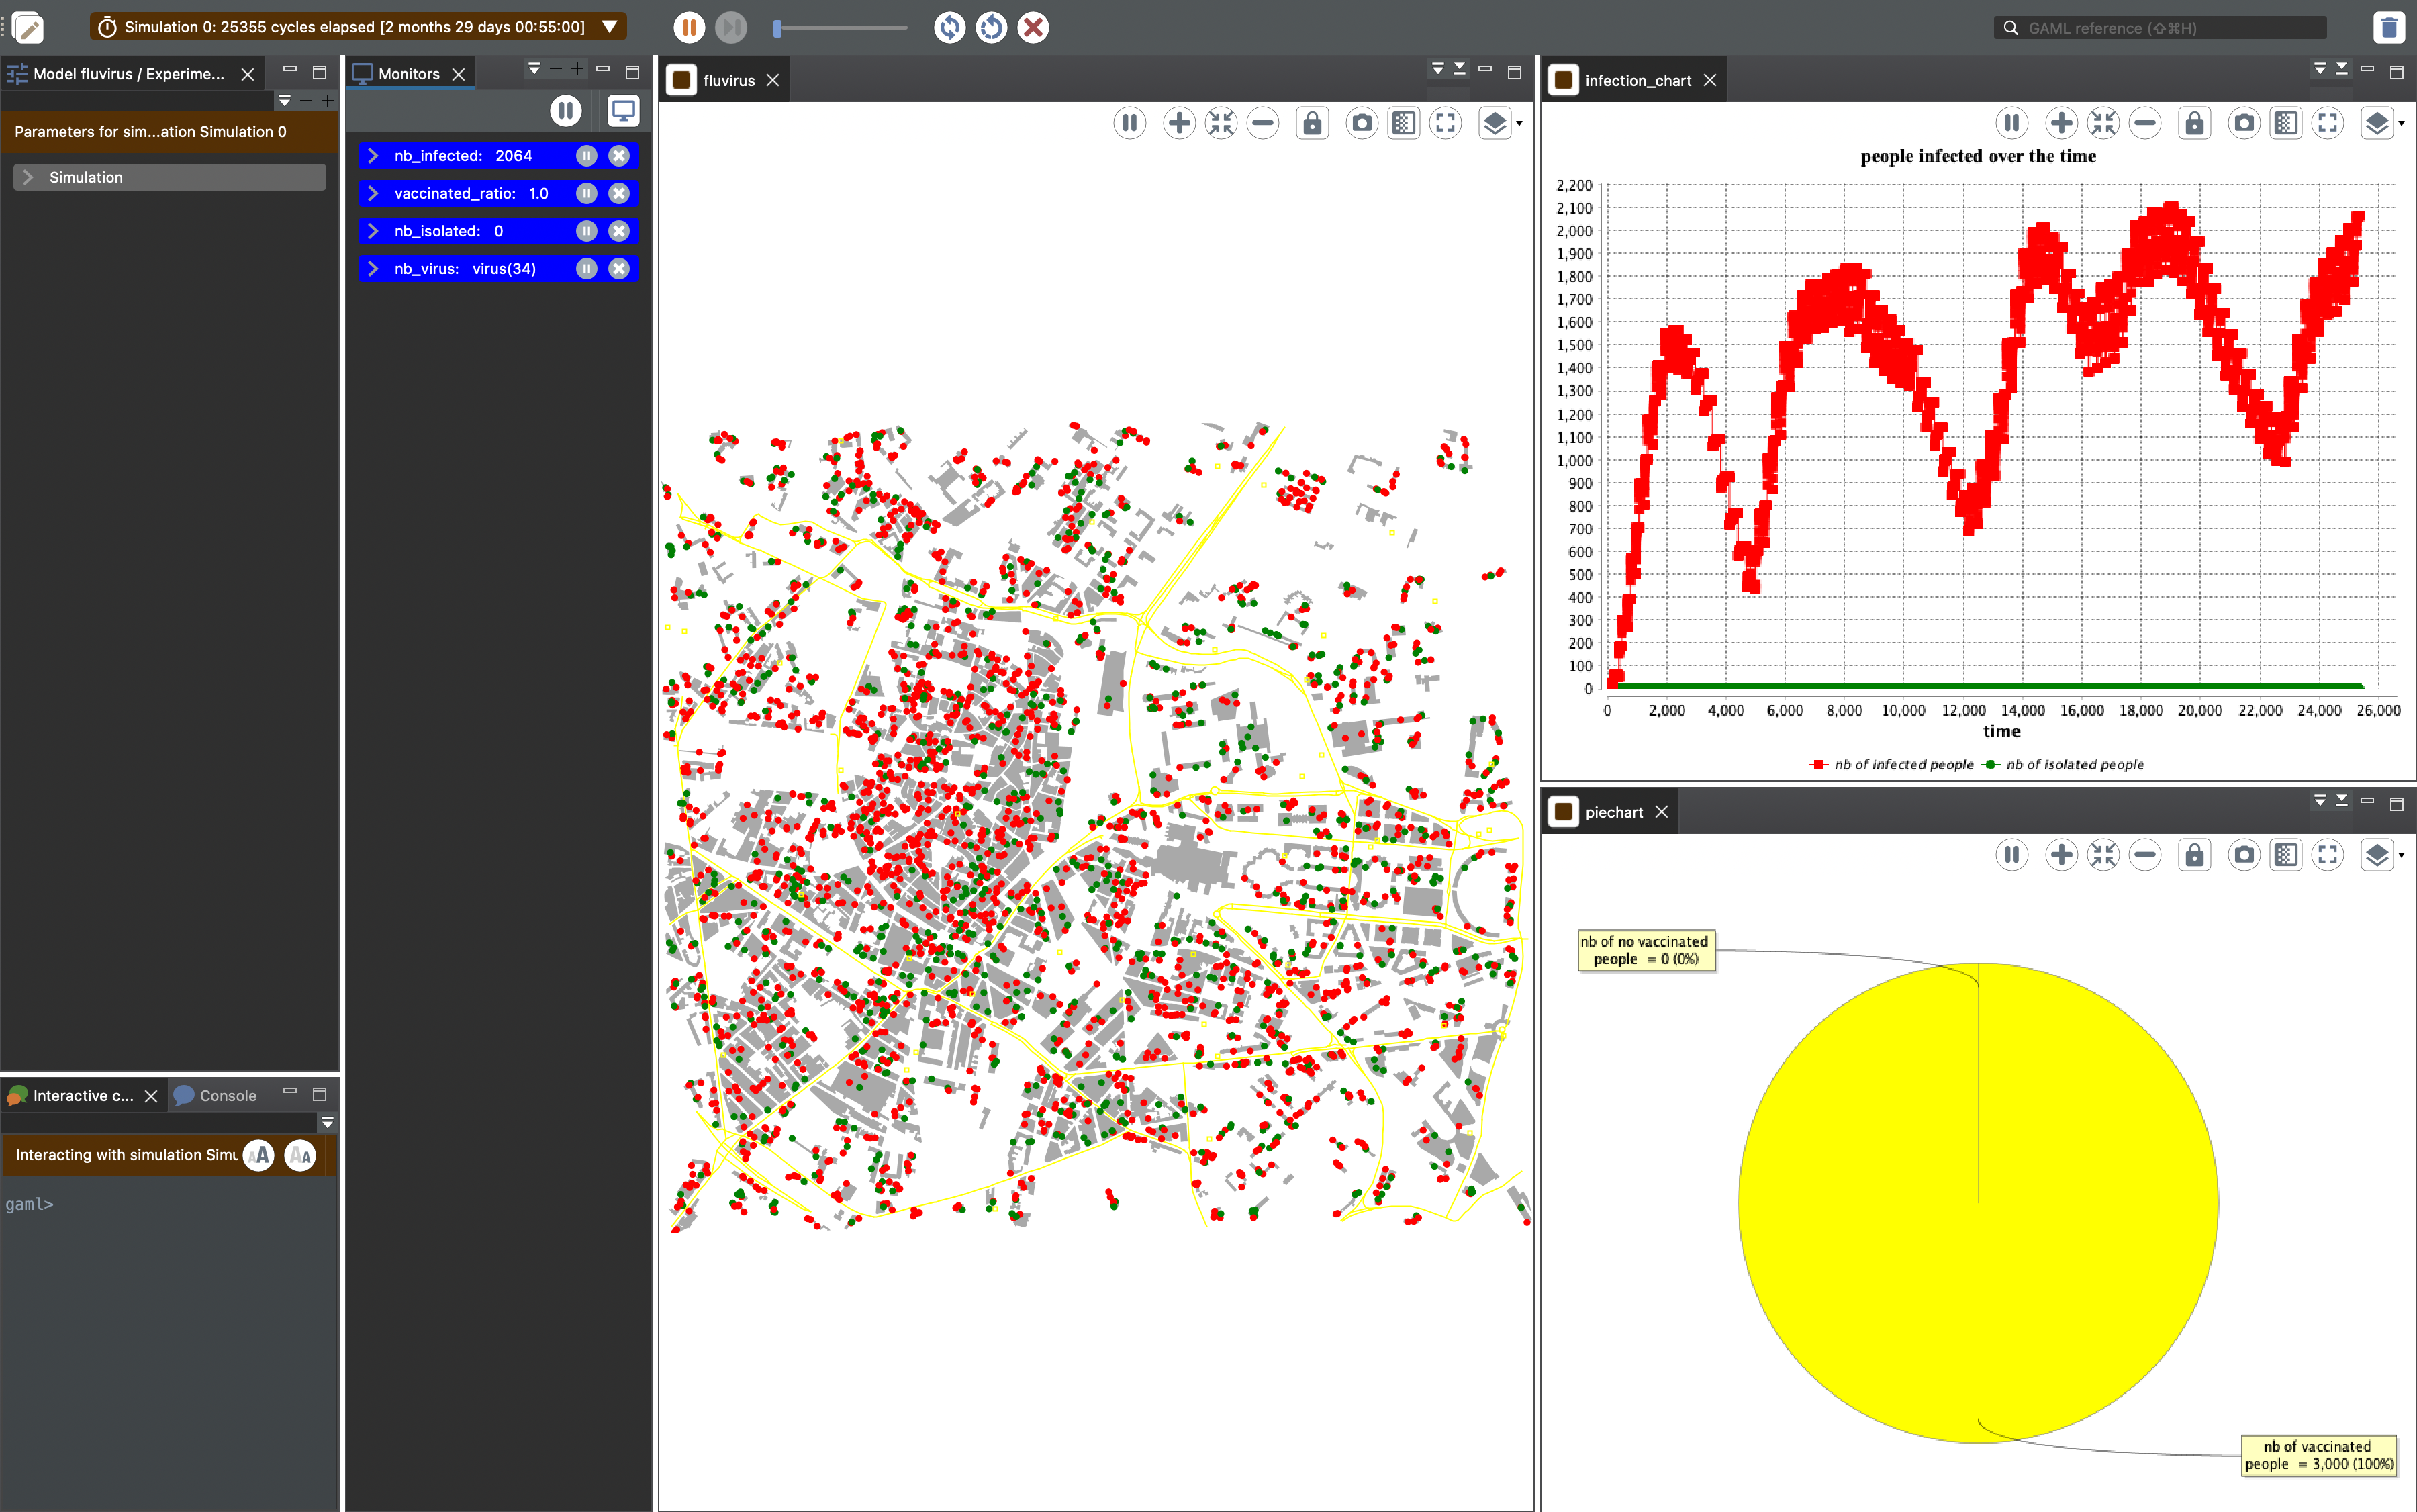
\includegraphics[width=0.8\textwidth]{images/imagecopy.png}
    \caption{Simulation results with a 10\% vaccination rate and no isolation.}
    \label{fig:simulation_vaccination_10}
\end{figure}

\paragraph{Key observations}
\begin{itemize}
    \item \textbf{Vaccination effect}: Increasing the vaccination rate reduces the intensity and frequency of infection peaks, but is not sufficient alone to control the epidemic without isolation measures.
    \item \textbf{Absence of isolation}: Without isolation, even a moderate vaccination rate cannot prevent recurring outbreaks.
    \item \textbf{Importance of combined strategies}: These simulations highlight the need for combining vaccination with isolation or other non-pharmaceutical interventions to effectively control the spread of the flu virus.
\end{itemize}

Overall, these results suggest that while increasing the vaccination rate helps mitigate the spread of the virus in opposite of the no isolation no vaccination scenario, relying solely on vaccination without isolation is insufficient to prevent large-scale outbreaks.

\section{Conclusion}
The simulations performed in this project illustrate the dynamics of flu virus propagation in an urban environment under different intervention strategies, including testing, isolation, and vaccination.

\paragraph{Notable Results:}
\begin{itemize}
    \item \textbf{Effectiveness of testing and isolation}: Increasing the daily testing rate and promptly isolating infected individuals significantly reduces the spread of the virus. In scenarios with testing rates of 20\% and 30\%, the epidemic curve showed faster containment and a shorter duration compared to scenarios without testing. However, isolation alone cannot fully prevent future outbreaks, as some infected individuals may not be detected early enough.
    
    \item \textbf{Impact of vaccination}: Introducing vaccination into the model demonstrated its ability to reduce the overall infection rate and flatten the epidemic curve. Even with a low vaccination rate of 5\% or 10\%, the intensity of the infection peaks decreased, showing the potential of vaccination to mitigate the epidemic. However, these low rates were insufficient to fully control the outbreak without complementary measures like isolation.

    \item \textbf{Combined strategies are critical}: The results emphasize that relying on a single strategy, such as vaccination or isolation alone, is not sufficient to effectively control an epidemic. Instead, a combination of strategies—high vaccination coverage, early testing, and isolation—is essential to prevent large-scale outbreaks and ensure long-term control of the virus.

    \item \textbf{No-intervention scenario}: The simulation with no vaccination and no isolation highlighted the risk of rapid and large-scale virus propagation. Without any intervention, the virus spread quickly, infecting a large proportion of the population, which emphasizes the importance of implementing timely measures during an outbreak.
\end{itemize}

\paragraph{Recommendations:}
Based on the simulations, it is recommended to:
\begin{enumerate}
    \item Increase vaccination coverage to at least 70\% of the population to achieve herd immunity and prevent recurring outbreaks.
    \item Maintain high daily testing rates as high as possible to detect and isolate infected individuals early, especially in the early phases of an epidemic.
    \item Combine vaccination with non-pharmaceutical interventions such as isolation and social distancing to ensure robust epidemic control.
\end{enumerate}

In conclusion, this project demonstrates the importance of adopting a multi-faceted approach to epidemic management. Further simulations could explore the effect of varying the vaccination rate, testing efficiency, and isolation duration to refine the intervention strategies.


\end{document}
